\section{Energieübertagung}\label{sec:Energie}
In diesem Kapitel wird aufgezeigt, wie die Energie übertragen werden soll. Die Schaltung auf der Primär- und der Sekundärseite werden entworfen.

\subsection{Konzept}
In der Abbildung \ref{fig:konzept_energie} sind die wichtigsten Komponenten der induktiven Energieübertragung aufgeführt. Rot umrandet sind die Komponenten die entwickelt werden müssen. Die Spannungsquelle und der Treiber für den Motor sind extern. Der Treiber bestimmt die zu übertragende Leistung von 300W und Gleichspannung von 48V.

\begin{figure}[h]
	\centering
	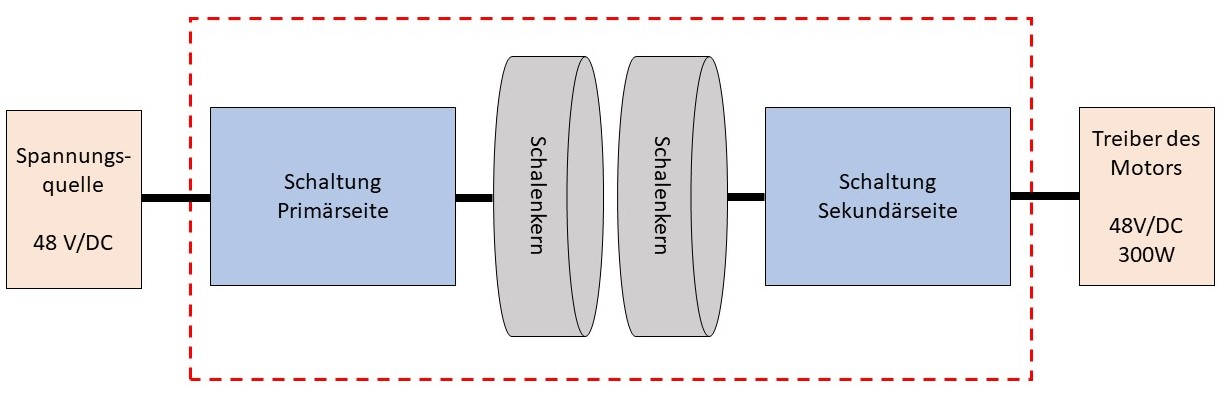
\includegraphics[width=1\linewidth]{konzept_energie}
	\caption{Konzept der induktiven Energieübertragung}\label{fig:konzept_energie}
\end{figure}

Die beiden Schalenkerne werden benötigt, um einen guten Kopplungsfaktor zu erreichen. Es sind Ferritkerne, welche aus dem Material BFM8 besteht und eine Anfangspermeabilität $ \mu_{i} $ von 2400 hat.\\ Die Schaltung auf der Primärseite hat die Aufgabe aus der Gleichspannung eine gepulste Spannung zu erzeugen, da keine konstante Spannung an der Spule anliegen darf. Wäre dies nicht der Fall könnte man keine Energie übertragen, denn das Magnetfeld der Spule würde sich nicht ändern und es würde keinen Strom in der zweiten Spule induziert. \\
Auf der sekundären Seite wird wieder eine gepulste Spannung erhalten. Aus dieser gepulsten Spannung soll die Sekundärschaltung wieder eine Gleichspannung kreieren.

\paragraph{Auswahl der Schaltungstopologie}
Für die Energieübertragung kommen verschiedene Typologien zu Frage. Der Flyback bringt interessante Vorteile mit sich. Im Vergleich zu anderen Schaltungen, welche eine galvanische Trennung beinhalten, benötigt er weniger Bauteile. Zusätzlich eignet sich die Schaltung für einen Leistungsbereich bis zu ca. 500W. Im Gegensatz zum Resonanzwandler muss der benötigte Transformator bestimmte Anforderungen erfüllen, da er gleichzeitig als Energiespeicher eingesetzt wird. Da es für einen Prototypen von Vorteil ist möglichst wenig Bauteile zu verwenden, fiel der Entscheid auf den Flyback-converter.\textcolor{red}{[Speerwandler, bachelor]}

In der Abbildung \ref{fig:konzept_flyback} wird die Schaltung des Flyback-converters aufgesplittet in die Primärschaltung, die Sekundärschaltung und die Schalenkerne. Die Primärseite besteht hauptsächlich aus dem MOSFET und dem Snubber-Glied. Die beiden Schalenkerene bilden den Speichertransformator, der für den Flyback benötigt wird. Die Sekundärschaltung ist ein Gleichrichter, welcher aus einer Schottky Diode und einem Kondensator gebildet wird.
\begin{figure}[h]
	\centering
	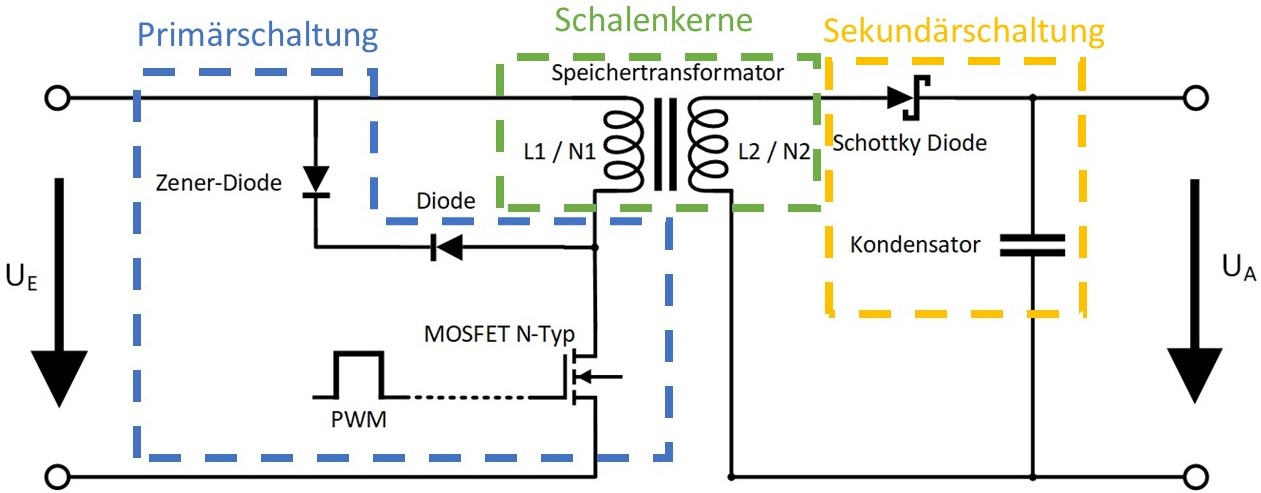
\includegraphics[width=0.9\linewidth]{konzept_flyback}
	\caption{Unterteilung der Flyback Schaltung}\label{fig:konzept_flyback}
\end{figure}


\subsection{Dimensionierung Flyback-converter}
Um den Flyback-converter simulieren und später in einem Testaufbau realisieren zu können, müssen die wichtigsten Komponenten ausgelegt werden. In diesen Abschnitt wird die Dimensionierung der Induktivität des Speichertransformators, des MOSFET, der Schottky Diode und der Snubber Schaltung erklärt. Die genauere Dimensionierung des Speichertransformators wird im Abschnitt \ref{sec:simulation} \refname{sec:simulation} genauer beschrieben.

\paragraph{Berechnung der Induktivität}
Ein wichtiger Wert um den Speichertransformator zu dimensionieren ist die Induktivität. Mit den beiden Formeln \ref{eq:energie} und \ref{eq:Leistung} lässt sich die übertragene Leistung $ P $ beschreiben. 

\begin{equation}\label{eq:zusammen}
P = \frac{1}{2} \cdot L \cdot \left (\frac{U_{E}}{L}\cdot a \cdot T_{p}\right ) ^{2} \cdot f_{p}
\end{equation}
Die Gleichung \ref{eq:zusammen} lässt sich nun nach der gesuchten Induktivität $ L $ umformen.
\begin{equation}\label{eq:induktivität}
L = \frac{a^{2}\cdot U_{E}\!^{2}\cdot T_{p}}{2 \cdot P}
\end{equation}

Mit einem Tastverhältnis $ a $ von 0.5, einer Eingangspannung $ U_{E} $ von 48V und der übertragenen Leistung $ P $ von 300W lässt sich die Induktivität berechnen. Die Periodendauer $ T_{p} $ ist variabel.

\begin{equation}\label{eq:induktivität_berechnet}
L = \frac{0.5^{2}\cdot 48\mathrm{V}^{2}\cdot T_{p}}{2 \cdot 300\mathrm{W}}
\end{equation}

In der Tabelle \ref{tab:induktivität} sind die berechneten Resultate der Induktivität in Abhängigkeit der Schaltfrequenz aufgeführt. Die Berechnungen geben Aufschluss darüber, dass die Induktivität kleiner werden muss, wenn die Frequenz erhört wird. Dies wird auch mit der Formel \ref{eq:strom} deutlich. In der Formel ist das Tastverhältnis, der Strom und die Spannung konstant. Wenn nun die Frequenz steigt, wird die Periodendauer kleiner und die Induktivität muss dementsprechend gesenkt werden.

\begin{table}[h]
	\centering
	\begin{tabular}{>{\tt}C{2.3cm}|  L{3cm}} 
		\normalfont\textbf{Frequenz} & \normalfont\textbf{Induktivität} \\ \hline\hline 
		10 kHZ & \SI{9.6e-05}{H}      \\ \hline
		20 kHZ & \SI{4.8e-05}{H}      \\ \hline
		30 kHZ & \SI{3.2e-05}{H}      \\ \hline
		40 kHZ & \SI{2.4e-05}{H}      \\ \hline
		50 kHZ & \SI{1.9e-05}{H}      \\ \hline
	\end{tabular}
\caption{Induktivität in Abhängigkeit der Schaltfrequenz }
\label{tab:induktivität}
\end{table}

\paragraph{Auslegung des MOSFET}
Die maximale Drain-Source-Spannung $ U_{DS} $ und der maximale Drain-Strom $ I_{D} $ sind wichtige Kenngrössen für die Auswahl des MOSFETs. Die grösste Spannung $ U_{DSmax} $ mit welcher der MOSFET belastet wird, berechnet sich mit der Formel \ref{eq:sperrspannung_mosfet}. Die Drain-Source-Spannung muss auf jeden Fall grösser $ U_{DSmax} $ gewählt werden.
\begin{equation}\label{eq:sperrspannung_mosfet}
U_{DSmax} = U_{e} + U_{a} \cdot \frac{N1}{N2}
\end{equation}
\begin{equation}\label{eq:sperrspannung_mosfet_berechnet}
U_{DSmax}= 48\mathrm{V} + 48\mathrm{V} \cdot 1 = 96\mathrm{V}
\end{equation}
\todo[inline]{ ev. Verlustleistung}

\paragraph{Auslegung des Ausgangsdiode}
Die Sperrspannung $ U_{R} $ der Schottky Diode muss folgendermassen ausgelegt werden.
\begin{equation}\label{eq:sperrspannung_diode}
U_{R} = U_{a} + U_{e} \cdot \frac{N2}{N1} = 48\mathrm{V} + 48\mathrm{V} \cdot 1 = 96\mathrm{V}
\end{equation}
\todo[inline]{ ev. Verlustleistung}

\paragraph{Auslegung  Snubber Schaltung}
Im Kapitel \ref{sec:Grundlagen} \refname{sec:Grundlagen} wurden zwei Snubber Schaltungen vorgestellt. Da der Aufbau mit einer Zener Diode und einer Diode (Abbildung \ref{fig:Flyback_zehner}) effizienter und zusätzlich unabhängig von der Streuinduktivität ist, fiel die Wahl auf diese Topologie. Die Durchbruch-Spannung $ U_{Z} $ der Zener Diode kann mit folgenden zwei Bedienungen festgelegt werden.  

\begin{equation}\label{eq:sperrspannung_zener1}
U_{Z} < U_{DS} - U_{E}
\end{equation}
\begin{equation}\label{eq:sperrspannung_zener1_berechnet}
U_{Z} <  150\mathrm{V} - 48\mathrm{V}  = 102\mathrm{V}
\end{equation}
\begin{equation}\label{eq:sperrspannung_zehner2}
U_{Z} > (U_{A} + U_{F}) \cdot \frac{N_{1}}{N_{2}}
\end{equation}
\begin{equation}\label{eq:sperrspannung_zehner2_berechnet}
U_{Z} >(48\mathrm{V} + 0.7\mathrm{V}) \cdot 1 = 48.7\mathrm{V}
\end{equation}
Die Durchbruch-Spannung darf also maximal 102 V betragen und mindestens 48.7 V.

\todo[inline]{Berechnung ev. Kondensator}

\subsection{Simulation}\label{sec:simulation}
Die Simulation der Schaltung sowie die erhaltenen Erkenntnisse aus der Simulation werden beschrieben.  

\paragraph{FEMM}
\todo[inline]{Infos zu Ferritkern}
\todo[inline]{Erwähnung von Sättigung}

\todo[inline]{Ziel 1: Anzahl Windungen Berechnen}
\todo[inline]{Tabelle Frequenzabhängig, Abstand, Windungen ==> Induktivität}

\begin{table}[h]
	\centering
	\begin{tabular}{C{1.5cm} C{2.3cm}|C{2cm} C{2.3cm} |C{2cm} C{2.3cm} }
		\multicolumn{2}{c|}{\textbf{}} & \multicolumn{2}{c|}{\textbf{1mm Distanz}}
		& \multicolumn{2}{c}{\textbf{0.1mm Distanz}} \\
		{Frequenz}& {Berechnet} &{Windungen}& {Induktivität} & {Windungen}& {Induktivität}\\ \hline\hline
		\multirow{2}{*}{10 kHz}  & \multirow{2}{*}{\SI{9.6e-05}{H}} & 11 & \SI{8.17E-05}{H}  & 4 & \SI{7.45E-05}{H}  \\
							    							      & & 12 & \SI{9.72E-05}{H}  & 5 & \SI{1.16E-04}{H}  \\ \hline
		\multirow{2}{*}{20 kHz}  & \multirow{2}{*}{\SI{4.8e-05}{H}} & 8 & \SI{4.33E-05}{H}  & 3 & \SI{4.19E-05}{H}  \\
												 & & 9 & \SI{5.48E-05}{H}  & 4 & \SI{7.45E-05}{H}  \\ \hline
		\multirow{2}{*}{30 kHz}  & \multirow{2}{*}{\SI{3.2e-05}{H}} & 6 & \SI{2.44E-05}{H}  & 2 & \SI{1.87E-05}{H}  \\
												 & & 7 & \SI{3.32E-05}{H}  & 3 & \SI{4.19E-05}{H}  \\ \hline
		\multirow{2}{*}{40 kHz}  & \multirow{2}{*}{\SI{2.4e-05}{H}} & \multirow{2}{*}{6} & \multirow{2}{*}{\SI{2.44E-05}{H}}  & 2 & \SI{1.234e3}{H}  \\
											     & &  &   & 3 & \SI{4.19E-05}{H}  \\ \hline
		\multirow{2}{*}{50 kHz}  & \multirow{2}{*}{\SI{1.9e-05}{H}} & 5 & \SI{1.70E-05}{H}  & \multirow{2}{*}{2} & \multirow{2}{*}{\SI{1.87E-05}{H}}  \\
												 & & 6 & \SI{2.44E-05}{H}  & &   \\ \hline
	\end{tabular}
	\caption{Resultate der Simulation in FEMM}\label{tab:windungen}
\end{table}


\todo[inline]{Ziel 2: Kopplungsfaktor Berechnen}
\todo[inline]{Ergebnis für 20, 30, ev. 50kHz}

Um mit FEMM die Selbstinduktion der Primär Spule zu ermitteln, lässt man einen Strom durch die Primär Wicklung und simuliert dies wie in Abbildung. Mit dem simulierten Fluss $ \Psi_{11}  $ und dem Strom $ I_{1} $ kann die Induktivität $ L_{1} $ wie folgt berechnet werden:

\begin{equation}
L_{1}=\frac{\Psi_{11}}{I_{1}}
\label{eq:femm_l1}
\end{equation}

Der Fluss $ \Psi_{1} $ lässt sich in FEMM simulieren in dem man durch die Primär und Sekundär einen Strom laufen lässt, wie in Abbildung. Mit der Formel \ref{eq:femm_M} wird die Gegeninduktivität $ M $ berechnet.

\begin{equation}
M=\frac{\Psi_{1}-\Psi_{11}}{I_{1}}=\frac{\Psi_{12}}{I_{1}}
\label{eq:femm_M}
\end{equation}

Da $ L_{1} $ und $ L_{2} $ den selben Wert besitzen kann man die Formel \ref{eq:kopplungsfaktor} vereinfachen wodurch sich nun der Kopplungsfaktor $ k $ wie folgt definiert:

\begin{equation}
k=\frac{M}{\sqrt{L_{1}^{2}}}
\label{eq:kopplungsfaktor_neu}
\end{equation}

%\begin{figure}
%\centering
%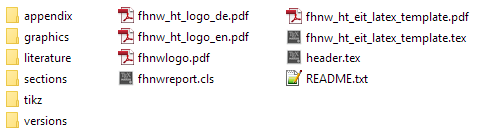
\includegraphics[width=0.8\linewidth]{ordner_struktur.png}
%\caption{FEMM-Simulation mit einem Strom durch die primär Wicklung}\label{fig:FEMM_1}
%\end{figure}


\begin{figure}[h]
	\centering
	\subfloat[Strom durch primär Wicklung.]{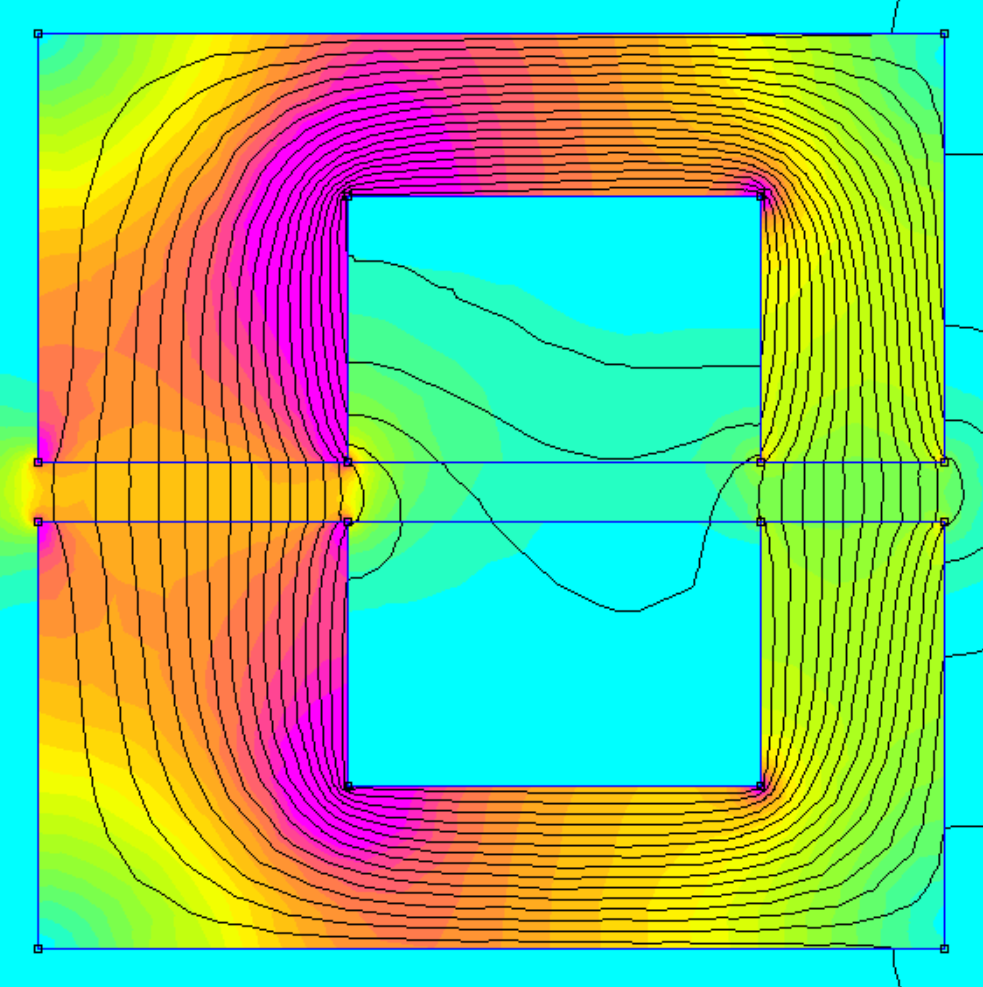
\includegraphics[width=0.45\linewidth]{femm_1.png}}\qquad
	\subfloat[Strom durch primär und sekundär Wicklung.]{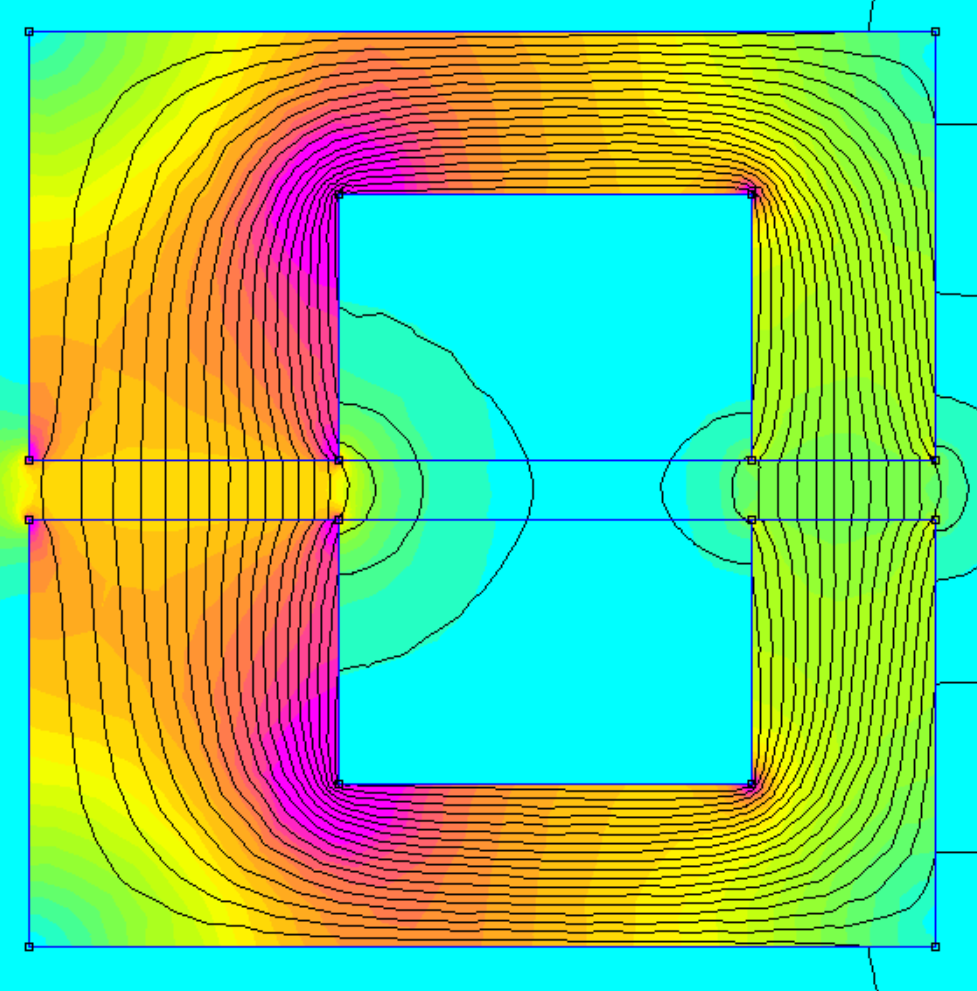
\includegraphics[width=0.45\linewidth]{femm_2.png}}
	\caption{Simulation des FEMM Models.}
	\label{fig:Subfigure}
\end{figure}

\paragraph{Schaltung}
\todo[inline]{Wirkungsgrad}
\todo[inline]{Energie}
\todo[inline]{Strom, Spannung}
\todo[inline]{Aufzeigen von Snubber}
\todo[inline]{Verlustleistung}

\subsection{Testaufbau}
\todo[inline]{Messung Induktivität, Widerstand, Freqeunzabhängig?}

\todo[inline]{Wirkungsgrad}
\todo[inline]{Energie}
\todo[inline]{Strom, Spannung}
\todo[inline]{Aufzeigen von Snubber}
\todo[inline]{Verlustleistung}